\documentclass[a4paper]{article}

\def\npart{III}
\def\nterm {Lent}
\def\nyear {2017-2018}
\def\nlecturer {Brian}
\def\ncourse {Decision}

\input{header}
\usetikzlibrary[topaths]
\usetikzlibrary{positioning,chains,fit,shapes,calc}
% A counter, since TikZ is not clever enough (yet) to handle
% arbitrary angle systems.
\newcount\mycount
\usepackage{verbatim}



\begin{document}

\maketitle

\tableofcontents

\section{Algorithms}
\subsection{Use an algorithm given in words}
\begin{eg}
The 'happy' algorithm is
\begin{itemize}
\item write down any integer
\item square its digits and find the sum of the squares
\item continue with this number
\item repeat until either the answer is 1 (happy) or until you get trapped in a cycle (not happy).
\end{itemize}
Show that
\begin{enumerate}
\item 70 is happy
\item 4 is unhappy
\end{enumerate}
\begin{proof}
\begin{enumerate}
\item \begin{align*} 7^2+0^2&=49 \\ 4^2+9^2 &= 96 \\ 9^2+7^2 &= 130 \\ 1^2+3^2 + 0^2 &=10 \\1^2 +0^2 &=1 \\ \text{so 70 is happy} \end{align*}
\item  \begin{align*} 4^2 &=16 \\ 1^2+6^2 &=37 \\ 3^2+7^2 &= 58 \\ 5^2+8^2 &= 89 \\ 1^2+4^2+5^2 &= 42 \\ 4^2+2^2 &= 20 \\ 2^2+0^2 &= 4 \\ 4^2 &=16 \\ \text{so 4 is unhappy} \end{align*}
\end{enumerate}
\end{proof}
\end{eg}

\begin{eg}
Implement this algorithm
\begin{itemize}
\item Let $n+1,A=1,B=1$ 
\item Write down A and B
\item Let $ C=A+B$
\item Write down C
\item Let $n=n+1,A=B,B=C$
\item If $n<5$ go to 3
\item If $n=5$ stop
\end{itemize}
\begin{proof}
\begin{centering}
\begin{tabular}{|c|c|c|c|c|c|}
\hline
Instruction step & n & A & B & C & Write down\\
\hline
1 & 1 & 1& 1 & & \\
\hline
2 & & & &  & 1,1 \\
\hline
3 & & & & 2& \\
\hline
4 & & & & &2 \\
\hline
5 & 2& 1& 2& & \\
\hline
6 & Go to step 3& \\
\hline
3 & & & &3 & \\
\hline
4 & & & & & 3\\
\hline
5 &3 &2 & 3& & \\
\hline
6 &Go to Step 3 \\
\hline
3 & & & & 5& \\
\hline
4 & & & & & 5\\
\hline
5 &4 &3 & 5& & \\
\hline
6 & Go to Step 3 \\
\hline
3 & & & &8 & \\
\hline
4 & & & & &8 \\
\hline
5 &5 & 5& 8& & \\
\hline
6 &Continue to Step 7\\
\hline
7 & Stop\\
\hline
\end{tabular}
\end{centering}
\end{proof}
\end{eg}

\begin{eg}
The algorithm multiplies the two numbers A and B.
\begin{itemize}
\item Make a table with two columns\\Write A in the top row of the left hand column and $B$ in the top row of the right hand column
\item In the next row of the table write: \begin{itemize}\item in the left hand column, the number that is half $A$, ignoring remainders \item in the right hand column the number that is double $B$ \end{itemize}
\item Repeat step 2 until you reach the row which has a 1 in the left hand column
\item Delete all rows where the number in the left hand column is even
\item Find the sum of the non-deleted numbers in the right hand column\\This is the product $AB$
\end{itemize}
Implement this algorithm when
\begin{enumerate}
\item $A=29$ and $B=34$
\item $A=66$ and $B=56$
\end{enumerate}
\begin{proof}
\begin{centering}
\begin{enumerate}
\item \begin{tabular}{|c|c|c|}
          \hline
          A&B& Step 4\\
          \hline
          14&68&Delete\\
          \hline
          7&136& \\
          \hline
          3&272 &\\
          \hline
          1&544 &\\
          \hline
          Total & 986&\\
          \hline          
          \end{tabular}
          So $29 \times 34 =986$
\item \begin{tabular}{|c|c|c|}
         \hline
          A&B&Step 4\\
          \hline
          66&56&Delete\\
          \hline
          33&112& \\
          \hline
          16&224&Delete \\
          \hline
          8&448&Delete \\
          \hline
          4&896&Delete \\
          \hline
          2&1792&Delete\\
          \hline
          1&3584&\\
          \hline
          Total & 3584&\\
          \hline          
          \end{tabular}
So $66\times56=3696$
\end{enumerate}
\end{centering}
\end{proof}
\end{eg}

\subsection{Implement an algorithm given in the form of a flow chat}
There are three shapes of boxes which are used in the examination\\
\begin{centering}
\includegraphics{img_D/2.png}
\end{centering}
\begin{eg}
\vspace{10pt}

\begin{enumerate}
\item Implement this algorithm using a trace table
\item Alter box 4 to read 'Let $E=3n$' and implement the algorithm again.
\end{enumerate}
How does this alter the algorithm?

\begin{proof}

\begin{enumerate}
\item \begin{tabular}{|c|c|c|}
          \hline
          n&E& box 6\\
          \hline
          14&68&no\\
          \hline
          7&136& no\\
          \hline
          3&272 &no\\
          \hline
          1&544 &no\\
          \hline
          Total & 986&no\\
          \hline          
          \end{tabular}
          
\item \begin{tabular}{|c|c|c|}
         \hline
          n&E&box 6\\
          \hline
          66&56&no\\
          \hline
          33&112& no\\
          \hline
          16&224&no \\
          \hline
          8&448&no \\
          \hline
          4&896&no \\
          \hline
          2&1792&no\\
          \hline
          1&3584&no\\
          \hline
          Total & 3584&no\\
          \hline          
          \end{tabular}

\end{enumerate}
\includegraphics[scale=0.4]{img_D/1.png}
\end{proof}

\end{eg}

\subsection{Bubble sort}
\subsection{Binary search}
\subsection{Implement the three bin packing algorithms}

\section{Graphs and networks}
\subsection{Basic Graph theory}
\begin{defi}[Vertices and Edges of Graph]
In the graph G, above
\begin{itemize}
\item the vertices (or nodes) are:
\item the edges (or arcs) are:
\end{itemize}
\end{defi}

\begin{defi}[Subgraph]
A subgraph of $G$ is a graph , each of whose vertices belongs to $G$ and each of whose edges belongs to $G$. It is simply a part of the original graph.
\end{defi}

\begin{defi}[Degree]
The degree or valency or order of a vertex is the number of edges incident to it
\end{defi}

\begin{prop}
If the degree of a vertex is even , we say it has even degree 
\end{prop}

\begin{defi}[Path]
A path is a finite sequence of edges, such that the end vertex of one edge in the sequence is the start vertex of the next, and in which no vertex appears more than once.
\end{defi}

\begin{defi}[Walk]
A walk is a path in which you are permitted to return to vertices more than once. 
\end{defi}

\begin{defi}[Cycle]
A cycle is a closed 'path'.
\end{defi}
\begin{tikzpicture}

\def \n {5}
\def \radius {3cm}
\def \margin {8} % margin in angles, depends on the radius

\foreach \s in {1,...,\n}
{
  \node[draw, circle] at ({360/\n * (\s - 1)}:\radius) {$\s$};
  \draw[->, >=latex] ({360/\n * (\s - 1)+\margin}:\radius) 
    arc ({360/\n * (\s - 1)+\margin}:{360/\n * (\s)-\margin}:\radius);
}
\end{tikzpicture}

\begin{defi}[Connected]
Two vertices are connected if there is a path between them. A graph is connected if all its vertices are connected.
\end{defi}

\begin{defi}[Loop]
A loop is an edge that starts and finishes at the same vertex
\end{defi}

\begin{defi}[Simple graph]
A simple graph is one in which there are no loops and not have more than one edge connecting any pair of vertices
\end{defi}

\begin{defi}[Digraph]
If the edges of a graph have a direction associated with them they are known as directed edges and the graph is known as a digraph.
\end{defi}

\begin{defi}[Tree]
A tree is a connected graph with no cycles
\end{defi}

\begin{defi}[Spanning tree]
A spanning tree of a graph ,$G$ is a subgraph which includes all the vertices of $G$ and is also a tree.
\end{defi}

\begin{defi}[Bipartite graph]
A bipartite graph consists of two sets of vertices , $X$ and $Y$. The edges only join vertices in $X$ to vertices in $Y$, not vertices within a set
\end{defi}

\begin{tikzpicture}[thick,
  fsnode/.style={},
  ssnode/.style={},
  every fit/.style={ellipse,draw,inner sep=5pt,text width=2cm},
  ->,shorten >= 3pt,shorten <= 3pt
]

% the vertices of U
\begin{scope}[start chain=going below,node distance=7mm]
\foreach \i/\xcoord/\ycoord in {1/6/8,2/5/1,3/-4/7,4/6/9,5/0/-3}
  \node[fsnode,on chain,label=left:$t_{\i}$] (f\i) {$(\xcoord,\ycoord)$};
\end{scope}

% the vertices of V
\begin{scope}[xshift=4cm,yshift=-0.5cm,start chain=going below,node distance=7mm]
\foreach \i/\xcoord/\ycoord in {6/0/3,7/1/4,8/-2/1,9/5/9}
  \node[ssnode,on chain,label=right:$t_{\i}$] (s\i) {$(\xcoord,\ycoord)$};
\end{scope}

% the set U
\node [mblue,fit=(f1) (f5),label=above:$X$] {};
% the set V
\node [mgreen,fit=(s6) (s9),label=above:$Y$] {};

% the edges
\draw (f1) -- (s6);
\draw (s6) -- (f2);
\draw (f2) -- (s7);
\draw (s7) -- (f3);
\draw (s8) -- (f3);
\draw (f3) -- (s9);
\draw (s9) -- (f5);
\draw (f5) -- (s6);
\end{tikzpicture}

\newpage

\begin{defi}[Complete graph]
A complete graph is a graph in which every vertex is directly connected by an edge to each of the other vertices. If the graph has $n$ vertices the connected graph is denoted by $K_n$.
\end{defi}

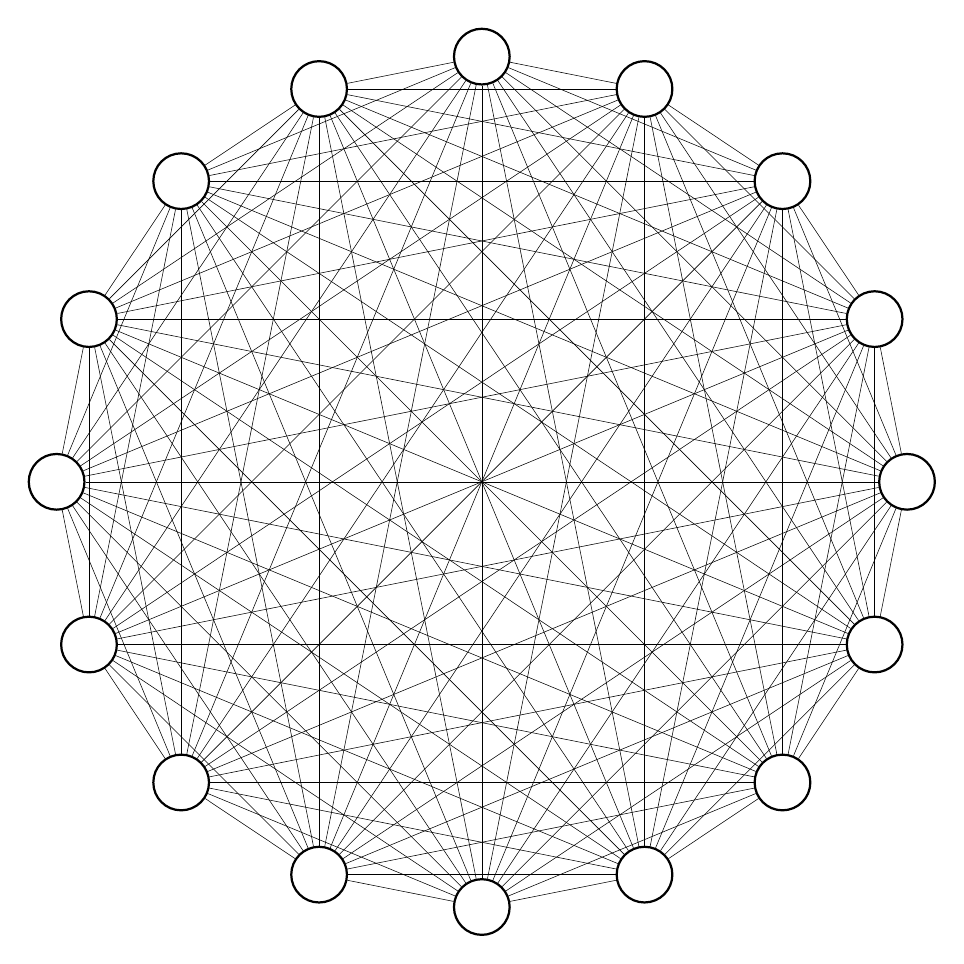
\begin{tikzpicture}[transform shape,line width=0.2pt]
  \foreach \x in {1,...,16}{%
    \pgfmathparse{(\x-1)*45+floor(\x/9)*22.5}
    \node[draw,circle,inner sep=0.25cm] (N-\x) at (\pgfmathresult:5.4cm) [thick] {};
  } 
  \foreach \x [count=\xi from 1] in {2,...,16}{%
    \foreach \y in {\x,...,16}{%
        \path (N-\xi) edge[-] (N-\y);
  }
}
\end{tikzpicture}

\begin{defi}[Complete bipartite graph]
A complete bipartite graph (denoted by $K_{r,s}$) in which there are $r$ vertices in set $X$ and $s$ vertices in set $Y$.
\end{defi}


\begin{defi}[Isomorphic graphs]
Isomorphic graphs are graphs that who the same information but are drawn differently
\end{defi}

\subsection{Adjacency Matrix and Distance matrix}
\begin{defi}[Adjacency Matrix]
A adjacency matrix records the number of direct links between vertices
\end{defi}

\begin{eg}
Use an adjacency matrix to represent this graph\\

\begin{tabular}{c|cccccc}
   &A&B&C&D&E&F\\
 \hline
 A&0&1&0&0&0&0\\
 B&1&0&1&0&2&1\\
 C&0&1&0&1&1&0\\
 D&0&0&1&0&0&1\\
 E&0&2&1&0&0&1\\
 F&0&1&0&1&1&2\\
\end{tabular}
\includegraphics{img_D/2_2ex1}
\end{eg}


\begin{defi}[Distance Matrix]
A distance matrix records the weights on the edges. Where there is no edge , we write '$-$'
\end{defi}
\begin{eg}
Use a distance matrix to represent this network.\\
\begin{tabular}{c|cccccc}
   &A&B&C&D&E&F\\
 \hline
 A&0&1&0&0&0&0\\
 B&1&0&1&0&2&1\\
 C&0&1&0&1&1&0\\
 D&0&0&1&0&0&1\\
 E&0&2&1&0&0&1\\
 F&0&1&0&1&1&2\\
\end{tabular}
\includegraphics{img_D/2_2ex2}
\end{eg}
\begin{eg}
Use a distance matrix to represent this directed network.\\
\begin{tabular}{c|ccccc}
   &A&B&C&D&E\\
 \hline
 A&-&17&18&-&-\\
 B&17&-&15&19&23\\
 C&18&15&-&20&-\\
 D&-&19&20&-&16\\
 E&-&23&-&16&-\\
\end{tabular}
\includegraphics{img_D/2_2ex3}
\end{eg}
\section{Algorithms on networks}
\subsection{Kruskal's algorithm}
Kruskal's algorithm finds the shortest, cheapest or fastest way of linking all the nodes into one system\\
You can use Kruskal's algorithm to find a minimum spanning tree.
\begin{defi}[Minimum spanning tree]
A minimum spanning tree (MST) is spanning tree such that the total length of its edges is as small as possible. (An MST is sometimes called a minimum connectors).
\end{defi}

\begin{defi}[Kruskal's algorithm]
Here is Kruskal's algorithm.
\begin{enumerate}
\item Sort all the edges into ascending order of weight.
\item Select the edges of least weight to start the tree
\item Consider the next edge of least weight.\begin{itemize}
                                                                       \item If it would form a cycle with the edges already selected, reject it. \item If it does not form a cycle, add it to the tree.
                                                                       \end{itemize}
                                                                       If there is choice of equal edges, consider each in turn.
\item Repeat step 3 until all vertices are connected.
\end{enumerate}

\end{defi}

\begin{eg}
Use Kruskal's algorithm to find a minimum spanning tree
\end{eg}

\begin{eg}

\end{eg}

\subsection{Prim's algorithm}
Like Kruskal's algorithm, Prim's algorithm finds the minimum spanning tree, but it uses a different approach.
\begin{defi}[Prim's algorithm]
Here is Prim's algorithm
\begin{enumerate}
\item Choose any vertex to start the tree.
\item \begin{itemize}
         \item Select an edges of least weight that joins a vertex that is already in the tree to a vertex that is not yet in the tree.
         \item If there is a choice of edges of equal weight , choose randomly.
         \end{itemize}
\item Repeat Step 2 until all the vertices are connected.
\end{enumerate}
\end{defi}

\begin{eg}

\end{eg}

You can apply Prim's algorithm to a distance matrix
\begin{defi}[Prim's algorithm to a distance matrix]
Here is the distance matrix form of Prim's algorithm
\begin{enumerate}
\item Choose any vertex to start the tree.
\item Delete the row in the matrix for the chosen vertex.
\item Number the column in the matrix for the chosen vertex
\item Put a ring round the lowest undeleted entry in the numbered columns. (If there is an equal choice, choose randomly.)
\item The ringed entry becomes the nest edge to be added to the tree.
\item Repeats steps 2,3,4 and 5 until all rows are deleted.
\end{enumerate}
\end{defi}

\begin{eg}
\begin{tabular}{c|ccccc}

\end{tabular}
\end{eg}

\subsection{Dijkstra's algorithm}
Dijkstra's algorithm is used to find the shortest, cheapest or quickest route between two vertices.

\begin{defi}[Dijkstra's algorithm]
Here is Dijkstra's algorithm\\
(to find the shortest path form $S$ to $T$ through a network).
\begin{enumerate}
\item Label the start vertex , $S$ , with the final label ,$0$.
\item Record a working value at every vertex , $Y$, that is directly connected to the vertex , $X$ , that has just received its final label.
\begin{itemize}
\item Working value at $Y=$ final value at $X+$ weight of arc $XY$
\item If there is already a working value at $Y$, it is only replaced if the new value is smaller.
\item Ince a vertex has a final label it is not revisited and its working values are no longer considered.
\end{itemize}
\item Look at the working values at all vertices without final labels. Select the smallest working value. This now becomes the final label at that vertex. (If two vertices have the same smallest working  value either may be given its final label first.)
\item Repeat steps 2 and 3 until the destination vertex , $T$, receives its final label.
\item To find the shortest path, trace back from $T$ to $S$. Given that $B$ already lies on the route, include arc $AB$ whenever final label of $B$ - final label of $A$ $=$ weight of arc $AB$. 
\end{enumerate}
\end{defi}
\begin{eg}

\end{eg}
\begin{eg}

\end{eg}
\begin{eg}

\end{eg}

\section{Route inspection (Chinese postman problem)}

\subsection{Traversable}

\begin{defi}[Eulerian]
If all the degrees in a graph are even, then the graph is Eulerian. If precisely two degrees are odd, and all the rest are even, then the graph is semi-Eulerian
\end{defi}

\begin{defi}[Traversable]
A graph is traversable if it is possible to traverse (travel along) every arc just once without taking your pen from the paper.

\end{defi}

\begin{prop}
A graph traversable if all the degrees are even
\end{prop}

\begin{prop}
A graph is semi-traversable if it has precisely two odd degrees. In this case the start point and the finish point will be the two vertices with odd degrees.
\end{prop}

\begin{prop}
A graph is not traversable if it has more than two odd degrees.
\end{prop}

\begin{eg}

\end{eg}

\begin{eg}

\end{eg}

\begin{eg}

\end{eg}

\subsection{Chinese postman algorithm (route inspection algorithm)}
You can use this algorithm to find the shortest route in a network that traverses every arc at least once and returns to the starting point.
\begin{prop}
If all the vertices have even degree the network is traversable. The length of the shortest route will be equal to the weight of the network 
\end{prop}
\begin{eg}

\end{eg}
\begin{prop}

\end{prop}
\begin{eg}

\end{eg}
\begin{eg}

\end{eg}

\begin{defi}[Route inspection algorithm]
Here is the route inspection algorithm
\begin{enumerate}
\item Identify any vertices with odd degree.
\item Consider all possible complete pairings of these vertices.
\item Select the complete pairing that has the least sum.
\item Add a repeat of the arcs indicated by this pairing to the network.
\end{enumerate}
\end{defi}

\begin{eg}

\end{eg}


\section{Critical path analysis}
\begin{eg}

\end{eg}

\section{Linear programming}

\section{Matchings}

\section{Transportation problems}

\section{Allocation (assignment) problems}

\section{The travelling salesman problem}

\section{Further linear programming}

\section{Game theory}

\section{Network flows}

\section{Dynamic programming}

\printindex

\end{document}